\subsection{Backpropagation}
The perceptron learning algorithm (see \ref{perceptron-training}) is not suitable for training FFNNs,
as it requires to compute the difference between the predicted output and the ground truth for each training example.
This is not possible for FFNNs, as in fact for hidden layers we don't have access to the true output, and we need to compute 
the error based on the output of the network and the true target variable.

To solve this problem, we can use the \textbf{Stochastic Gradient Descent} (SGD) algorithm, in combination with the \textbf{backpropagation} algorithm, 
which allows to efficiently compute the gradients of the loss function with respect to the parameters of the network.
\subsubsection{Idea behind Backpropagation}
Before backpropagation, a few ideas were proposed to learn the weights inside a FFNN:
\begin{itemize}
    \item \textbf{Randomly perturb the weights}: randomly perturb one weight at a time and check
    if the loss function decreases. This is inefficient and does not scale well with the number of parameters in the network.
    \item \textbf{Parallel Perturbation}: randomly perturb all the weights at the same time and check if the loss function decreases.
    This doesn't help at all, as we would need many perturbations to get a good estimate of the gradient;
    \item \textbf{Perturb the activations}: randomly perturb the activations of the hidden layers and check if the loss function decreases. 
    This is more efficient than perturbing the weights, as we have fewer activations than weights, but it still does not scale well with the number of parameters in the network.
\end{itemize}
From the last idea, the backpropagation algorithm was born, which instead measure how the loss function changes with respect to the activations of the hidden layers.

\subsubsection{The algorithm}
The backpropagation algorithm, introduced in the section \ref{introduction-backpropagation}, consists of three main steps:
\begin{itemize}
    \item \textbf{Forward Pass}: compute the output of the network for a given input $\boldsymbol{x}$ and the current parameters $\boldsymbol{\theta}$;
    \item \textbf{Error Computation}: compute the error at the output layer by comparing the predicted output with the true target variable $y$;
    \item \textbf{Backward Pass}: propagate the error signal back through the network, allowing to update the parameters of the network using the computed gradients.
\end{itemize}
As said before, we cannot know from the training data what the expected output of the hidden units should be, but we can compute how
the error changes with respect to the change in the hidden units.

\subsubsection{Single Neuron Case}
Let's first consider a neural network with just one neuron in each layer.
After performing the forward pass, we can express the output of the network as follows:
\begin{equation*}
    a^{(L)} = \sigma(z^{(L)}) = \sigma(w^{(L)} a^{(L-1)} + b^{(L)})
\end{equation*}
where $a^{(L)}$ is the output of the last layer, $\sigma$ is a non-linear activation function, 
$w^{(L)}$ and $b^{(L)}$ are respectively the weight and bias of the last layer, and $a^{(L-1)}$ is the output of the previous layer.

Our goal is to understand how a small change in the parameters $w^{(l)}$ will affect the loss function $\mathcal{L}$.
When computing this, we need to consider the chain of dependencies between the parameters and the loss function:
\begin{itemize}
    \item How a change in $w^{(l)}$ affects the output of the layer $z^{(l)}$;
    \item How a change in $z^{(l)}$ affects the output of the layer $a^{(l)}$;
    \item How a change in $a^{(l)}$ affects the loss function $\mathcal{L}$.
\end{itemize}
This is where the chain rule of calculus comes into play, allowing us to compute the gradient of the 
loss function with respect to the parameters by multiplying the gradients along the chain of dependencies.

Formally, we can express the gradient of the loss function with respect to the parameters $w^{(l)}$ as follows:
\begin{equation*}
    \frac{\partial \mathcal{L}}{\partial w^{(l)}} = \frac{\partial z^{(l)}}{\partial w^{(l)}} \cdot \frac{\partial a^{(l)}}{\partial z^{(l)}} \cdot \frac{\partial \mathcal{L}}{\partial a^{(l)}}
\end{equation*}
where respectively:
\begin{itemize}
    \item $\frac{\partial z^{(l)}}{\partial w^{(l)}}$ measures how a small change in the weight $w^{(l)}$ affects the output of the layer $z^{(l)}$;
    \item $\frac{\partial a^{(l)}}{\partial z^{(l)}}$ measures how a small change in the output of the layer $z^{(l)}$ affects the output of the activation function $a^{(l)}$;
    \item $\frac{\partial \mathcal{L}}{\partial a^{(l)}}$ measures how a small change in the output of the activation function $a^{(l)}$ affects the loss function $\mathcal{L}$.
\end{itemize}
The process can be extended to deeper layers. In those cases, we need to consider the chain of dependencies from the parameter we want to update
to the output of the network, computing the gradients along the way using the chain rule of calculus.
\begin{figure}[H]
    \centering
    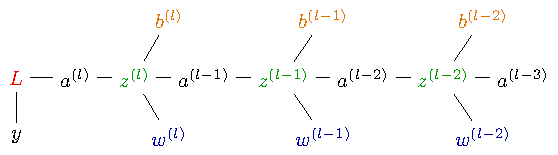
\includegraphics[width=\textwidth]{chapters/02-ffnn/media/dependencies.pdf}
    \caption{Dependency chain for a parameter in a deep network.}
\end{figure}
Taking in consideration the architecture shown in the figure above, we can express the derivative of the loss function with respect to a parameter $w^{(l-1)}$ in a deeper layer as follows:
\begin{equation*}
    \frac{\partial \mathcal{L}}{\partial w^{(l-1)}} = \frac{\partial z^{(l-1)}}{\partial w^{(l-1)}} \cdot \frac{\partial a^{(l-1)}}{\partial z^{(l-1)}} \cdot \underbrace{\frac{\partial z^{(l)}}{\partial a^{(l-1)}} \cdot \frac{\partial a^{(l)}}{\partial z^{(l)}} \cdot \frac{\partial \mathcal{L}}{\partial a^{(l)}}}_{\frac{\partial \mathcal{L}}{\partial a^{(l-1)}}}
\end{equation*}
\subsubsection{General Case}
The general case of backpropagation doesn't differ much from the single neuron case. We simply have to consider all the possible
way in which a change in a parameter can affect the loss function, and compute the gradients accordingly using the chain rule of calculus.

To take into account the fact that each layer can have multiple neurons, we also need to update the notation. Since each connection in the network has its own weight,
we represent with $w_{ij}^{(l)}$ the weight connecting the $j$-th neuron in layer $l-1$ to the $i$-th neuron in layer $l$.

The weighted sum for the $i$-th neuron in layer $l$ can be expressed as follows:
\begin{equation*}
    z_i^{(l)} = \sum_{j} w_{ij}^{(l)} a_j^{(l-1)} + b_i^{(l)}
\end{equation*}
where $a_j^{(l-1)}$ is the output of the $j$-th neuron in the previous layer, and $b_i^{(l)}$ is the bias term for the $i$-th neuron in layer $l$.

When we consider the output layer neurons, the chain of dependencies remains the same as in the single neuron case, as each output neuron is directly connected to the loss function.
\begin{equation*}
    \frac{\partial \mathcal{L}}{\partial w_{ij}^{(L)}} = \frac{\partial z_i^{(L)}}{\partial w_{ij}^{(L)}} \cdot \frac{\partial a_i^{(L)}}{\partial z_i^{(L)}} \cdot \frac{\partial \mathcal{L}}{\partial a_i^{(L)}}
\end{equation*}

For the hidden layer neurons, we instead need to consider all the possible paths from the parameter we want to update to the output layer, and compute the gradients accordingly.
\begin{figure}[H]
    \centering
    \scalebox{0.5}{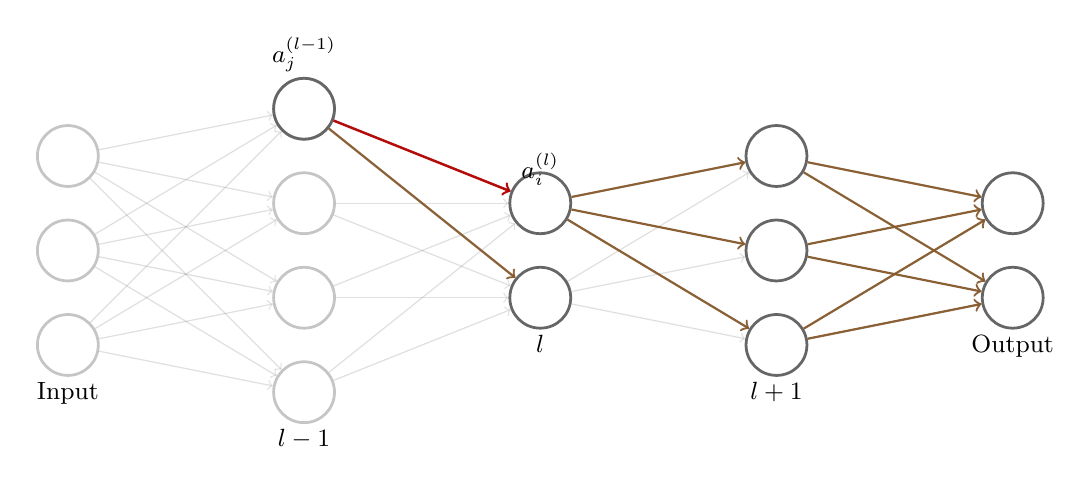
\begin{tikzpicture}[
  neuron/.style={circle, draw=black!60, line width=1.0pt, minimum size=22pt, inner sep=0pt},
  faded_neuron/.style={neuron, opacity=0.38},
  focus_neuron/.style={neuron, opacity=1.0},
  conn_faded/.style={->, draw=black!55, line width=0.45pt, opacity=0.22},
  conn_active/.style={->, draw=brown!70!black, line width=0.8pt, opacity=0.95},
  conn_weight/.style={->, draw=red!70!black, line width=0.9pt, opacity=0.95}
]

% Input layer (faded)
\foreach \i/\y in {1/1.2,2/0,3/-1.2} {
  \node[faded_neuron] (i\i) at (0, \y) {};
}

% Hidden layer 1 (top node in focus, rest faded)
\foreach \j/\y in {1/1.8,2/0.6,3/-0.6,4/-1.8} {
  \node[faded_neuron] (h1\j) at (3.0, \y) {};
}
\node[focus_neuron] (h11f) at (3.0, 1.8) {};

% Hidden layer 2 (both nodes in focus)
\foreach \j/\y in {1/0.6,2/-0.6} {
  \node[focus_neuron] (h2\j) at (6.0, \y) {};
}

% Hidden layer 3 (all in focus)
\foreach \j/\y in {1/1.2,2/0,3/-1.2} {
  \node[focus_neuron] (h3\j) at (9.0, \y) {};
}

% Output layer (in focus)
\foreach \k/\y in {1/0.6,2/-0.6} {
  \node[focus_neuron] (o\k) at (12.0, \y) {};
}

% --- Faded dense connections ---
\foreach \i in {1,...,3} {
  \foreach \j in {1,...,4} {
    \draw[conn_faded] (i\i) -- (h1\j);
  }
}
\foreach \i in {1,...,4} {
  \foreach \j in {1,...,2} {
    \draw[conn_faded] (h1\i) -- (h2\j);
  }
}
\foreach \i in {1,...,2} {
  \foreach \j in {1,...,3} {
    \draw[conn_faded] (h2\i) -- (h3\j);
  }
}
\foreach \i in {1,...,3} {
  \foreach \k in {1,2} {
    \draw[conn_faded] (h3\i) -- (o\k);
  }
}

% --- Highlighted path ---
% Red weight: h11f -> h21 and h11f -> h22
\draw[conn_weight] (h11f) -- (h21);
\draw[conn_active] (h11f) -- (h22);

% Brown active: from h21 -> all of HL3
\foreach \j in {1,...,3} {
\draw[conn_active] (h21) -- (h3\j);
}

% Brown active: all of HL3 -> all outputs
\foreach \i in {1,...,3} {
  \foreach \k in {1,2} {
    \draw[conn_active] (h3\i) -- (o\k);
  }
}

% --- Labels ---
\node[above=4pt]  at (3.0,  2)  {\small $a_j^{(l-1)}$};
\node[below=4pt]  at (6.0, 1.5)  {\small $a_i^{(l)}$};
\node[below=10pt] at (0,   -1.2)  {\small Input};
\node[below=10pt] at (3.0, -1.8)  {\small $l-1$};
\node[below=10pt] at (6.0, -0.6)  {\small $l$};
\node[below=10pt] at (9.0, -1.2)  {\small $l+1$};
\node[below=10pt] at (12.0,-0.6)  {\small Output};

\end{tikzpicture}}
    \caption{Dependency chain for a parameter feeding into $h_2$.}
    \label{fig:backpropagation_output}
\end{figure}
\begin{equation*}
    \frac{\partial \mathcal{L}}{\partial a_j^{(l-1)}} = \sum_{i} \frac{\partial z_i^{(l)}}{\partial a_j^{(l-1)}} \cdot \frac{\partial a_i^{(l)}}{\partial z_i^{(l)}} \cdot \frac{\partial \mathcal{L}}{\partial a_i^{(l)}}
\end{equation*}